\chapter{\MM}
\label{chap:mm}

\MM is an extension of the MLton~\cite{MLton} compiler and runtime system that
targets scalable, multicore architectures. MLton is a whole-program optimizing
compiler for Standard ML programming language, which a member of the ML family
of programming languages that includes Objective Caml and F\#. Apart from \MM,
another notable example in the multicore ML space is
Manticore~\cite{Fluet2007}, and focuses on implicit parallelism under an
ML-inspired language. In this chapter, we will present the programming model
and the runtime system details of \MM, which provides the technical background
that informs the rest of the dissertation.

\section{Programming Model}

While MLton does not target multicore processors, it does include excellent
support for Concurrent ML (CML)~\cite{Reppy99}, a concurrent extension of
Standard ML that utilizes synchronous message passing to enable to construction
of synchronous communication protocols. The programming model supported by \MM
is heavily influenced by CML. We begin by briefly describing the CML
programming model, before its extension used in \MM.

\subsection{Concurrent ML}

Concurrent ML~\cite{Reppy99} is a concurrent extension of Standard ML with
support for user-level thread creation, where the threads primarily interact by
performing synchronous \cf{send} and \cf{recv} operations on typed channels;
these operations block until a matching actions on the same channel is
performed by a different thread.

CML also provides first-class synchronous {\em events} that abstract
synchronous message-passing operations.  An event value of type \cf{'a Event}
when synchronized on yields a value of type \cf{'a}.  An event value represents
a potential computation, with latent effect until a thread synchronizes upon it
by calling \cf{sync}. The following equivalences thus therefore hold:
\cf{send(c, v)} $\equiv$ \cf{sync(sendEvt(c,v))} and \cf{recv(c)} $\equiv$
\cf{sync(recvEvt(c))}. Notably, thread creation is {\em not} encoded as an
event -- the thread \cf{spawn} primitive simply takes a thunk to evaluate as a
separate thread, and returns a thread identifier that allows access to the
newly created thread's state.

Besides \cf{sendEvt} and \cf{recvEvt}, there are other base events provided by
CML\@.  The \cf{never} event, as its name suggests, is never available for
synchronization; in contrast, \cf{alwaysEvt} is always available for
synchronization.  These events are typically generated based on the
(un)satisfiability of conditions or invariants that can be subsequently used to
influence the behavior of more complex events built from the event combinators
described below.  Much of CML's expressive power derives from event combinators
that construct complex event values from other events.  We list some of these
combinators below:
\vspace{5mm}

\lstset{numbers=none}
\begin{lstlisting}
spawn     : (unit -> 'a) -> threadID
sendEvt   : 'a chan * 'a -> unit Event
recvEvt   : 'a chan -> 'a Event
alwaysEvt : 'a -> 'a Event
never     : 'a Event
sync      : 'a Event -> 'a
wrap      : 'a Event * ('a -> 'b) -> 'b Event
guard     : (unit -> 'a Event) -> 'a Event
choose    : 'a Event list -> 'a Event
\end{lstlisting}

The expression \cf{wrap (ev, f)} creates an event that, when synchronized,
applies the result of synchronizing on event \cf{ev} to function \cf{f}.
Conversely, \cf{guard(f)} creates an event that, when synchronized, evaluates
\cf{f()} to yield event \cf{ev} and then synchronizes on \cf{ev}.  The
\cf{choose} event combinator takes a list of events and constructs an event
value that represents the non-deterministic choice of the events in the list;
for example:
\vspace{5mm}

\lstset{numbers=none}
\begin{lstlisting}
sync(choose[recvEvt(a),sendEvt(b,v)])
\end{lstlisting}

\noindent will either receive a unit value from channel \cf{a}, or send value
\cf{v} on channel \cf{b}.  Selective communication provided by \cf{choose}
motivates the need for first-class events. We cannot, for example, simply build
complex event combinators using function abstraction and composition because
function closures do not allow inspection of the encapsulated computations, a
necessary requirement for implementing combinators like \cf{choose}.

\subsection{Asynchronous Concurrent ML}

While simple to reason about, synchronous events impose non-trivial performance
penalties, requiring that both parties in a communication action be available
before allowing either to proceed.  To relax this condition, \MM allows the
expression of \emph{asynchronous} composable events, through an asynchronous
extension of concurrent ML (\acml).

An asynchronous operation initiates two temporally distinct sets of actions.
The first defines {\em post-creation} actions -- these are actions that must be
executed after an asynchronous operation has been initiated, without taking
into account whether the effects of the operation have been witnessed by its
recipients.  For example, a post-creation action of an asynchronous send on a
channel might initiate another operation on that same channel; the second
action should take place with the guarantee that the first has already
deposited its data on the channel.  The second are {\em post-consumption}
actions -- these define actions that must be executed only after the effect of
an asynchronous operation has been witnessed.  For example, a post-consumption
action might be a callback that is triggered when the client retrieves data
from a channel sent asynchronously.  These post-consumption actions take place
within an implicit thread of control responsible for completing the
asynchronous operation.

\acml introduces first-class {\em asynchronous} events with the following
properties: {\emph (i)} they are extensible both with respect to pre- and
post-creation as well as pre- and post-consumption actions; {\emph (ii)} they
can operate over the same channels that synchronous events operate over,
allowing both kinds of events to seamlessly co-exist; and, {\emph (iii)} their
visibility, ordering, and semantics is independent of the underlying runtime
and scheduling infrastructure.

In order to provide primitives that adhere to the desired properties outlined
above, \acml extends CML with a new asynchronous event type \cf{('a,'b) AEvent}
and the following two base events: \cf{aSendEvt} and \cf{aRecvEvt}, to create
an asynchronous send event and an asynchronous receive event, respectively. The
differences in their type signature from their synchronous counterparts reflect
the split in the creation and consumption of the communication action they
define:
\vspace{5mm}

\lstset{numbers=none}
\begin{lstlisting}
sendEvt  : 'a chan * 'a -> unit Event
recvEvt  : 'a chan -> 'a Event
aSendEvt : 'a chan * 'a -> (unit, unit) AEvent
aRecvEvt : 'a chan -> (unit, 'a) AEvent
\end{lstlisting}

An \cf{AEvent} value is parameterized with respect to the type of the event's
post-creation and post-consumption actions.  In the case of \cf{aSendEvt}, both
actions yield \cf{unit}: when synchronized on, the event immediately returns a
\cf{unit} value and places its \cf{'a} argument value on the supplied channel.
The post-consumption action also yields \cf{unit}. When synchronized on, an
\cf{aRecvEvt} returns \cf{unit}; the type of its post-consumption action is
\cf{'a} reflecting the type of value read from the channel when it is paired
with a send. The semantics of both asynchronous send and receive guarantees
that successive communication operations performed by the same thread get
witnessed in the order in which they were issued.

Beyond these base events, \acml also provides a number of combinators that
serve as asynchronous versions of their CML counterparts. These combinators
enable the extension of post-creation and post-consumption action of
asynchronous events to create more complex events, and allow transformation
between the synchronous and asynchronous events.
\vspace{2mm}

\lstset{numbers=none}
\begin{lstlisting}
wrap  : 'a Event * ('a -> 'b) -> 'b Event
sWrap : ('a, 'b) AEvent * ('a -> 'c) -> ('c, 'b) AEvent
aWrap : ('a, 'b) AEvent * ('b -> 'c) -> ('a, 'c) AEvent

guard  : (unit -> 'a Event) -> 'a Event
aGuard : (unit -> ('a, 'b) AEvent) -> ('a, 'b) AEvent

choose  : 'a Event list -> 'a Event
aChoose : ('a, 'b) AEvent list -> ('a, 'b) AEvent
sChoose : ('a, 'b) AEvent list -> ('a, 'b) AEvent

aTrans : ('a, 'b) AEvent -> 'a Event
sTrans : 'a Event -> (unit, 'a) AEvent
\end{lstlisting}

Similar to CML \cf{wrap} combinator, \cf{sWrap} and \cf{aWrap} extend the
post-consumption and post-creation actions of an asynchronous event,
respectively. \cf{aGuard} allows creation of a guarded asynchronous event.
\cf{sChoose} is a blocking choice operator which blocks until one of the
asynchronous base events has been consumed. \cf{aChoose} is a non-blocking
variant, which has the effect of non-deterministically choosing one of the base
asynchronous events if none are available for immediate consumption. Finally,
\cf{aTrans} and \cf{sTrans} allow transformation between the synchronous and
asynchronous variants.
\vspace{5mm}

\lstset{numbers=none}
\begin{lstlisting}
sync  : 'a Event -> 'a
aSync : ('a, 'b) AEvent -> 'a
\end{lstlisting}

We also introduce a new synchronization primitive: \cf{aSync}, to synchronize
asynchronous events. The \cf{aSync} operation fires the computation
encapsulated by the asynchronous event of type \cf{('a, 'b) AEvent}, returns a
value of type \cf{'a}, corresponding to the return type of the event's
post-{\em creation} action. Unlike their synchronous variants, asynchronous
events do {\em not} block if no matching communication is present.  For
example, executing an asynchronous send event on an empty channel places the
value being sent on the channel and then returns control to the executing
thread. In order to allow this non-blocking behavior, an {\em implicit} thread
of control is created for the asynchronous event when the event is paired, or
{\em consumed}. If a receiver is present on the channel, the asynchronous send
event behaves similarly to a synchronous event; it passes the value to the
receiver. However, a new implicit thread of control is still created to execute
any post-consumption actions.

Similarly, the synchronization of an asynchronous receive event does not yield
the value received; instead, it simply enqueues the receiving action on the
channel. Therefore, the thread that synchronizes on an asynchronous receive
always gets the value {\tt unit}, even if a matching send exists. The actual
value consumed by the asynchronous receive can be passed back to the thread
which synchronized on the event through the use of combinators that process
post-consumption actions.  This is particularly well suited to encode reactive
programming idioms: the post-consumption actions encapsulate a reactive
computation.

Further details about the \MM programming model and \acml can be found
in~\cite{Ziarek11}.

\section{Compiler}

Since the concurrent programming model of \MM is exposed as a library on top of
MLton, \MM retains MLton's compiler infrastructure, and only adds a few
additional compiler primitives for concurrency support. \MM is a whole-program
optimizing compiler for the full SML 97 language~\cite{SML97}, including
modules and functors. During compilation, \MM first transforms the source
program with modules and functors into an equivalent one without by
defunctorization~\cite{ElsmanPhD}. Defunctorization duplicates each functor at
every application and eliminates structures by renaming variables. Next, the
program is monomorphized~\cite{Reynolds1972} by instantiating the polymorphic
datatypes and functions at every application. The program is then
defunctionalized, replacing the higher-order functions with data structures to
represent them and first-order functions to apply them. The resultant
intermediate language is in Static Single Assignment (SSA)
form~\cite{Bilardi2003}. Much of the aggressive optimizations are performed in
SSA passes. The SSA code is then transformed to RSSA intermediate
representation. RSSA is similar SSA, but exposes data representations decisions
that leads to further optimizations. The compiler can produce native code for
multiple backends as well as portable C output.

\section{Runtime System}

\subsection{Threading System}

\MM's runtime system is specifically optimized for efficiently handling the
large number of concurrent threads, both implicit and explicit, created by the
\acml programming model. \MM uses an {\em m} over {\em n} threading system that
leverages potentially many lightweight (language level) threads multiplexed
over a collection of kernel threads. The user-level thread scheduler is in turn
implemented using the \cf{MLton.Thread}~\cite{MLton} library, which provides
one-shot continuations. \cf{MLton.Thread} uses a variation of Bruggeman
\emph{et al}.'s~\cite{Bruggeman1996} strategy for implementing one-shot
continuations. A \cf{MLton.Thread} is a lightweight data structure that
represents a paused computation, and encapsulates the metadata associated with
the thread as well as a stack. The stack associated with the lightweight thread
is allocated on the heap, and is garbage collected when the corresponding
thread object is no longer reachable.

As such, \cf{MLton.Thread} does not include a default scheduling mechanism.
Instead, \MM builds a preemptive, priority supported, run-queue based,
multicore-capable scheduler using \cf{MLton.Thread}. Building multicore
schedulers over continuations in this way is not new, first described by Wand
et al.~\cite{ContMP}, and successfully emulated by a number of modern language
implementations~\cite{ghc,Auhagen11}. Each core has a private scheduler queue,
and new threads are by default spawned on the same core. The programmer can
explicitly request for a thread to be spawned on a different core. However,
once spawned, the threads remain pinned to their cores.

Implementing \MM's threading system over one-shot continuation as opposed to
full-fledged (multi-shot) continuations greatly reduces the cost of the thread
and scheduler implementation. In particular, if full-fledged continuations were
used to implement the scheduler, then during every thread switch, a
\emph{copy} of the current thread would have to be made to reify the
continuation. This is, in our context, unnecessary since the current stack of
the running thread (as opposed to the saved stack in the continuation), will
never be accessed again.  One-shot continuations avoid
copying the stack altogether; during a thread switch, a reference to the
currently running thread is returned to the programmer. The result is a very
efficient baseline scheduler.

Lightweight threads are garbage collected when no longer reachable. \MM's
threading system multiplexes many lightweight thread on top of a few operating
system threads. Each kernel thread represents a virtual processor and one
kernel thread is pinned to each processor. The number of kernel threads is
determined statically and is specified by the user; they are not created during
program execution.

While lightweight threads provide a conceptually simple language mechanism for
asynchrony, they are unsuitable for expressing the implicit asynchronous
threads created by the \acml programming model. This is due to the
synchronization, scheduling, and garbage collection costs associated with
lightweight threads, which outweigh the benefit of running the computation
concurrently. With the aim of carrying out \acml's implicit asynchronous
actions, \MM supports a new threading mechanism called \emph{parasitic
threads}. Thus, our runtime supports two kinds of threads: hosts and parasites.
Host threads map directly to lightweight threads in the runtime. Parasitic
threads can encapsulate arbitrary computation, just like host threads. However,
unlike a regular thread, a parasitic thread executes using the execution
context of the host that creates the parasite; it is intended primarily to
serve as the execution vehicle for asynchronous actions.

Parasitic threads are implemented as raw frames living within the stack space
of a given host thread.  A host thread can hold an arbitrary number of
parasitic threads. In this sense, a parasitic thread views its host in much the
same way as a user-level thread might view a kernel-level thread that it
executes on. A parasite is suspended when it performs a blocking action (e.g.,
a synchronous communication operation, or I/O). Such a suspended parasite is
said to have been \emph{reified}. Reified parasites are represented as stack
objects on the heap. Reified parasites can resume execution once the conditions
that had caused it to block no longer hold. Thus, parasitic threads are not
scheduled using the language runtime; instead they \emph{self-schedule} in a
demand-driven style based on flow properties dictated by the actions they
perform.

\begin{figure}[t]
\begin{center}
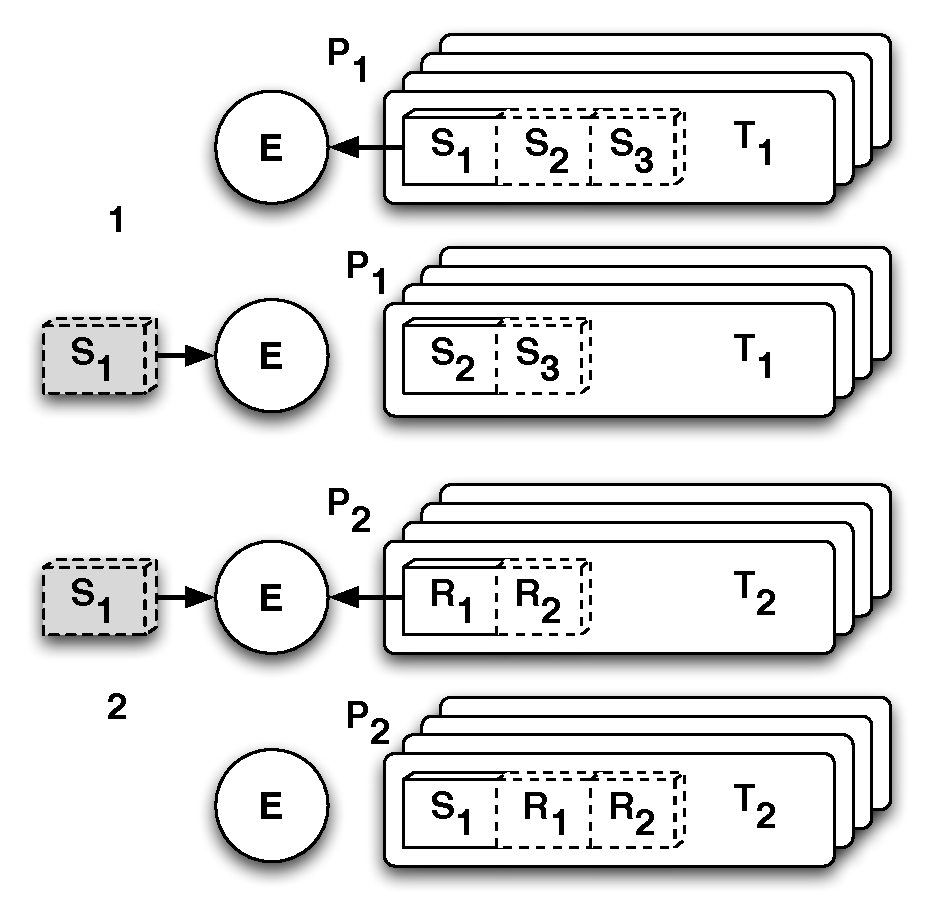
\includegraphics[scale=0.4]{Figures/communication.pdf}
\end{center}
\caption{Blocking and unblocking of parasitic threads.}
\label{fig:block_unblock}
\end{figure}

Figure~\ref{fig:block_unblock} shows the steps involved in a parasitic
communication, or blocking event, and we illustrate the interaction between the
parasitic threads and their hosts. The host threads are depicted as rounded
rectangles, parasitic threads are represented as blocks within their hosts, and
each processor as a queue of host threads. The parasite that is currently
executing on a given host and its stack is represented as a block with solid
edges; other parasites are represented as blocks with dotted edges. Reified
parasites are represented as shaded blocks. Host threads can be viewed as a
collection of parasitic threads all executing within the same stack space. When
a host thread is initially created it contains one such computation, namely the
expression it was given to evaluate when it was spawned.

Initially, the parasite \cf{$S_1$} performs a blocking action on a channel or
event, abstractly depicted as a circle. Hence, \cf{$S_1$} blocks and is
reified. The thread \cf{$T_1$} that hosted \cf{$S_1$} continues execution by
switching to the next parasite \cf{$S_2$}. \cf{$S_1$} becomes runnable when it
is unblocked. Part 2 of the figure shows the parasite \cf{$R_1$} on the thread
\cf{$T_2$} invoking an unblocking action. This unblocks \cf{$S_1$} and
schedules it on top of \cf{$R_1$}. Thus, the parasitic threads implicitly
migrate to the point of synchronization.

Further details about parasitic threads including its operational semantics and
mapping of \acml primitives to parasitic threads can be found in~\cite{JFP14}.

\subsection{Garbage Collector}
\label{sec:gc}

\MM garbage collector (GC) is optimized for throughput. It uses a single,
contiguous heap, shared among all the cores, with support for local allocation
and stop-the-world collection. In order to allow local allocation, each core
requests a page-sized chunk from the heap. While a single lock protects the
chunk allocation, objects are allocated within chunks by bumping a core-local
heap frontier.

In order to perform garbage collection, all the cores synchronize on a barrier,
with one core responsible for collecting the entire heap. The garbage
collection algorithm is inspired from Sansom's~\cite{Sansom91} collector, which
combines Cheney's two-space copying collector and Jonker's single-space sliding
compaction collector. Cheney's copying collector walks the live objects in the
heap just once per collection, while Jonker's mark-compact collector performs
two walks. But Cheney's collector can only utilize half of memory allocated for
the heap. Sansom's collector combines the best of both worlds. Copying
collection is performed when heap requirements are less than half of the
available memory. The runtime system dynamically switches to mark-compact
collection if the heap utilization increases beyond half of the available
space.

Since ML programs tend to have a high rate of allocation, and most objects are
short-lived temporaries, it is beneficial to perform generational collection.
The garbage collector supports Appel-style generational
collection~\cite{Appel89} for collecting temporaries. The generational
collector has two generations, and all objects that survive a generational
collection are copied to the older generation. Generational collection can work
with both copying and mark-compact major collection schemes.

\MM enables its generational collector only when it is profitable, which is
determined by the following heuristic. At the end of a major collection, the
runtime system calculates the ratio of live bytes to the total heap size. If
this ratio falls below a certain (tunable) threshold, then generational
collection is enabled for subsequent collections. By default, this ratio is
0.25.
